\documentclass[11pt]{article}
\usepackage[margin=2.5cm]{geometry}
\usepackage{graphicx}
\usepackage{booktabs}
\usepackage{amsmath}
\usepackage{natbib}
\usepackage{hyperref}
\usepackage{microtype}
\usepackage{parskip}
\usepackage{setspace}
\usepackage{array}
\usepackage{caption}

\graphicspath{{../experiment_v2/figures/}}

\hypersetup{
  colorlinks=true,
  linkcolor=blue,
  citecolor=blue,
  urlcolor=blue
}

\title{\textbf{Perception Over Adoption: Perceived AI Job Threat Predicts\\
Developer Job Satisfaction More Strongly than AI Tool Use}\\[0.4em]
\large Evidence from the 2024 Stack Overflow Developer Survey}

\author{Anonymous Author}
\date{}

\begin{document}

\maketitle

% -----------------------------------------------------------------------
\begin{abstract}
The integration of artificial intelligence tools into software development has
prompted claims that AI adoption drives developer productivity and well-being.
Using data from the 2024 Stack Overflow Developer Survey ($N = 17{,}696$),
this study tests whether perceived AI job threat or actual AI tool adoption
is a stronger predictor of developer job satisfaction.
Ordinary least-squares regression and group-comparison analyses reveal that
developers who perceive AI as a threat to their jobs report significantly lower
job satisfaction than those who do not ($d = 0.33$, $\eta^2 = 0.012$,
$p < 10^{-47}$), with a mean difference of 0.67 points on a 0--10 scale.
By contrast, whether developers currently use AI tools is effectively
unrelated to job satisfaction ($d = 0.031$, $p = 0.14$).
The AIThreat effect persists after controlling for experience, remote-work
status, and organisation size ($\beta = -0.65$, $p < 10^{-44}$), and holds
equally among current AI tool users.
These results suggest that psychological threat perception, not adoption
behaviour, is the mechanism linking AI to developer job satisfaction.
\end{abstract}

% -----------------------------------------------------------------------
\section{Introduction}

Artificial intelligence coding assistants have moved from novelty to daily
infrastructure in professional software development. Industry surveys
consistently report that a large majority of developers have experimented
with or adopted tools such as GitHub Copilot, ChatGPT, or similar assistants
\citep{vaillant2024developers}. The dominant narrative accompanying this shift
is that AI adoption increases productivity and, by extension, developer
well-being: more capable tools should translate into more satisfying work.

Yet adoption rates and subjective well-being need not move together.
A growing body of research suggests that the \emph{psychological response} to
AI—rather than its practical use—may be the more consequential variable.
\citet{sadeghi2024employee} finds that AI deployment in organisational
settings simultaneously raises concerns about employment stability, fairness,
and privacy, with the net effect on worker contentment dependent on
implementation context rather than on whether employees use the technology.
At the societal level, \citet{giuntella2025ai} show, using longitudinal German
panel data, that workers in highly AI-exposed occupations do not report lower
life satisfaction or greater job insecurity than comparable workers in
less-exposed roles—suggesting that aggregate exposure by itself is not harmful.
For individual well-being, however, the picture appears different: \citet{feng2025ai}
demonstrate that AI-related workplace anxiety directly reduces life satisfaction
through heightened negative affect, with social support acting as a buffer.

In a systematic review of 92 workplace AI studies,
\citet{soulami2024exploring} identify \emph{workplace autonomy} and
\emph{psychological health} as the two most consistently observed mediating
themes: AI adoption affects employees primarily through changes in perceived
control and stress, not through raw exposure or tool usage per se.
These findings collectively point toward a hypothesis that has received
little direct empirical testing in the software development domain:
that \emph{perceived AI threat}, rather than \emph{AI adoption status},
is the dominant predictor of developer job satisfaction.

The present study tests this hypothesis using data from the 2024 Stack
Overflow Developer Survey, one of the largest annual samples of software
professionals worldwide. Specifically, we ask:

\begin{quote}
\textit{Does perceived AI job threat predict lower developer job satisfaction,
and does this effect exceed the effect of actual AI tool adoption?}
\end{quote}

Our null hypothesis~($H_0$) is that AIThreat does not predict job satisfaction
after controlling for AI tool adoption and standard covariates ($\beta = 0$).
The alternative~($H_1$) is that AIThreat is a significant negative predictor
($\beta < 0$, $d \geq 0.25$) and that its effect substantially exceeds that
of adoption behaviour.

% -----------------------------------------------------------------------
\section{Methodology}

\subsection{Data Source}

Data are from the \emph{2024 Stack Overflow Annual Developer Survey},
a publicly available cross-sectional survey of software developers worldwide.
The full dataset contains 65{,}437 responses. The primary outcome variable
is \textsc{JobSat} (0--10, integer), answered by 29{,}126 respondents
(55.5\,\% item non-response). Exploratory analyses indicate that non-response
to \textsc{JobSat} is concentrated among hobby coders and students
(i.e.\ respondents without a professional employment context), suggesting a
Missing~At~Random (MAR) pattern conditional on MainBranch.

\subsection{Analytic Sample}

The analytic sample was restricted to respondents who (a)~provided a
\textsc{JobSat} value, (b)~gave a binary response to \textsc{AIThreat}
(``Yes'' or ``No''; ``I'm not sure'' and ``NA'' excluded from primary analysis),
(c)~reported a current or near-term \textsc{AISelect} status (``Yes'' or
``No, but I plan to soon''), and (d)~had valid values for all covariates
(RemoteWork, OrgSize). This yielded $N = 17{,}696$.

\subsection{Variables and Encoding}

\textbf{Outcome.} \textsc{JobSat}: continuous 0--10 (higher = more satisfied).

\textbf{Primary predictor.} \textsc{AIThreat\_Yes}: 1 if the respondent views
AI as a threat to their job, 0 otherwise (reference: No).

\textbf{Secondary predictor.} \textsc{AISelect\_Yes}: 1 if the respondent
currently uses AI tools, 0 if they plan to use them soon (reference).
Note: within the AIThreat Yes/No subsample, the category
``No, and I don't plan to'' is absent, so the reference becomes
``plans to use soon.''

\textbf{Covariates.} YearsCodePro (continuous; 21.1\,\% missing, imputed with
sample median of~8 years under the MAR assumption), RemoteWork (three dummies;
reference: In-person), OrgSize (eight dummies; reference: Freelancer / just me).

\subsection{Statistical Analysis}

We conducted (1)~Welch $t$-tests and one-way ANOVA with $\eta^2$ for bivariate
comparisons; (2)~OLS regression in two nested models---Model~1 (AIThreat +
AISelect without covariates) and Model~2 (full model)---to assess $\beta$
coefficients, $R^2$, and incremental $\Delta R^2$; (3)~Cohen's~$d$ for
standardised effect sizes; (4)~variance inflation factors (VIF) to assess
multicollinearity; and (5)~a robustness check restricted to current AI tool
users ($n = 14{,}538$). Effect-size interpretation follows Cohen's conventions
($d \geq 0.20$ small, $\geq 0.50$ medium; $f^2 \geq 0.02$ small, $\geq 0.15$ large).

% -----------------------------------------------------------------------
\section{Results}

\subsection{Descriptive Statistics}

Table~\ref{tab:descriptives} reports means and standard deviations for the
two AIThreat groups and the two AISelect groups.

\begin{table}[h]
\centering
\caption{Descriptive statistics for \textsc{JobSat} by AIThreat and AISelect.}
\label{tab:descriptives}
\small
\begin{tabular}{lrrrr}
\toprule
Group & $n$ & Mean & SD & Median \\
\midrule
\multicolumn{5}{l}{\textit{AIThreat}} \\
AIThreat = No  & 15{,}414 & 7.099 & 2.025 & 7 \\
AIThreat = Yes &  2{,}282 & 6.426 & 2.285 & 7 \\
\midrule
\multicolumn{5}{l}{\textit{AISelect}} \\
Currently uses AI   & 14{,}538 & 7.024 & 2.089 & 7 \\
Plans to use AI     &  3{,}158 & 6.960 & 1.994 & 7 \\
\bottomrule
\end{tabular}
\end{table}

The mean difference between AIThreat groups is 0.67 points on the 0--10 scale.
The mean difference between AISelect groups is only 0.06 points.

\subsection{Primary Analysis: AIThreat vs.\ AISelect}

\begin{figure}[h]
  \centering
  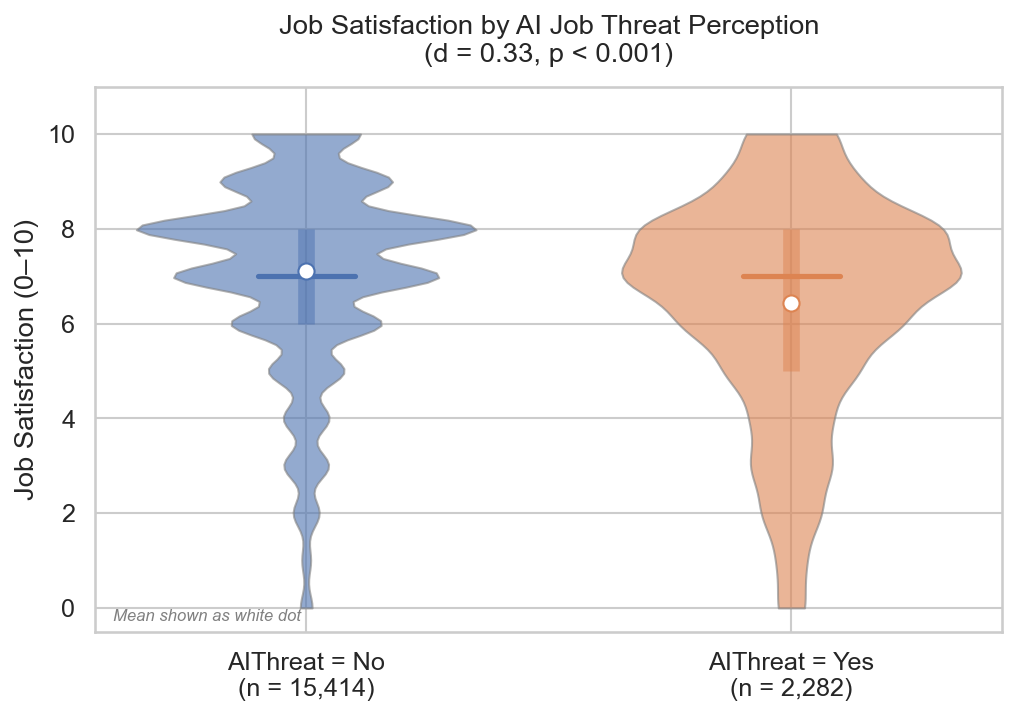
\includegraphics[width=0.62\textwidth]{fig1_jobsat_by_aithreat.png}
  \caption{Distribution of \textsc{JobSat} by AIThreat group.
           Violin plot with embedded box (IQR); white dots denote group means.
           $d = 0.33$, $p < 10^{-47}$.}
  \label{fig:violin}
\end{figure}

A Welch $t$-test confirmed a significant mean difference between AIThreat
groups ($t = 13.32$, $p < 2.5 \times 10^{-39}$, Figure~\ref{fig:violin}).
One-way ANOVA yielded $F(1, 17{,}694) = 212.27$, $p < 8.3 \times 10^{-48}$,
$\eta^2 = 0.012$. The standardised effect size was Cohen's $d = 0.33$
(small-to-moderate range), compared to $d = 0.031$ for AISelect (negligible).

\begin{figure}[h]
  \centering
  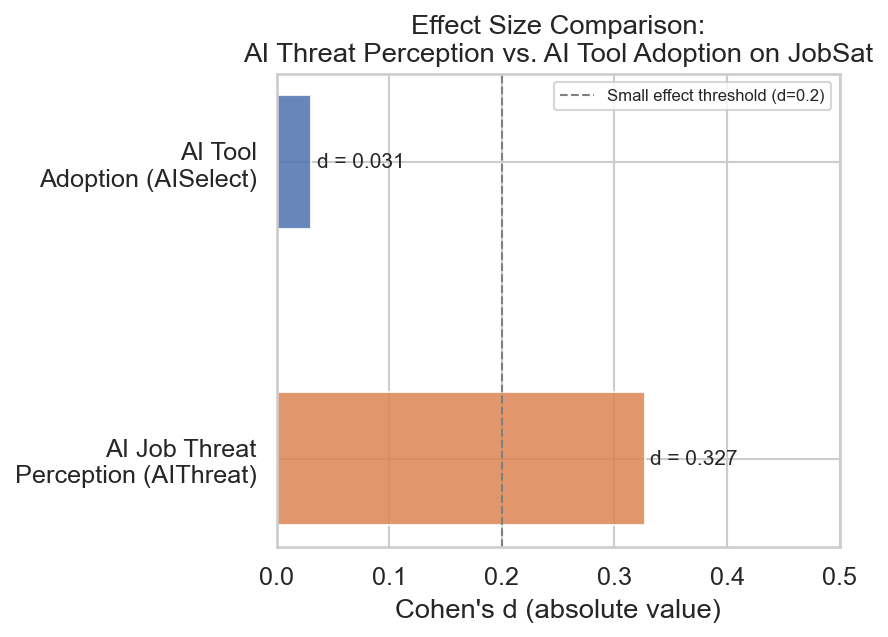
\includegraphics[width=0.62\textwidth]{fig3_effect_size_comparison.png}
  \caption{Effect-size comparison (Cohen's $d$): AIThreat vs.\ AISelect.
           Dashed line marks the conventional small-effect threshold ($d = 0.20$).}
  \label{fig:effectsize}
\end{figure}

Figure~\ref{fig:effectsize} visualises this contrast directly: AIThreat
exceeds the small-effect threshold by a factor of~1.6, while AISelect
falls far below it.

\subsection{Regression Analysis}

Table~\ref{tab:regression} presents the two OLS models.

\begin{table}[h]
\centering
\caption{OLS regression predicting \textsc{JobSat}. Reference categories:
AIThreat=No, AISelect=Plans-to-use, RemoteWork=In-person, OrgSize=Freelancer.}
\label{tab:regression}
\small
\begin{tabular}{lrrrr}
\toprule
 & \multicolumn{2}{c}{Model 1} & \multicolumn{2}{c}{Model 2} \\
\cmidrule(lr){2-3}\cmidrule(lr){4-5}
Predictor & $\beta$ & $p$ & $\beta$ & $p$ \\
\midrule
Intercept         &  7.050 & $<$0.001 & 6.644 & $<$0.001 \\
AIThreat\_Yes     & $-$0.673 & $<$0.001 & $-$0.651 & $<$0.001 \\
AISelect\_Yes     & 0.060  & 0.140    & 0.096 & 0.018 \\
YearsCodePro      & ---    & ---      & 0.028 & $<$0.001 \\
RemoteWork\_Hybrid & ---   & ---      & 0.242 & $<$0.001 \\
RemoteWork\_Remote & ---   & ---      & 0.336 & $<$0.001 \\
OrgSize dummies   & ---    & ---      & n.s.\ (mostly) & --- \\
\midrule
$N$  & \multicolumn{2}{c}{17{,}696} & \multicolumn{2}{c}{17{,}696} \\
$R^2$ & \multicolumn{2}{c}{0.012} & \multicolumn{2}{c}{0.033} \\
\bottomrule
\end{tabular}
\end{table}

In Model~1, AIThreat\_Yes carries a coefficient of $\beta = -0.673$
($p < 0.001$; 95\,\%~CI: $[-0.763, -0.582]$), while AISelect\_Yes is
non-significant ($\beta = 0.060$, $p = 0.14$). After adding all covariates
in Model~2, AIThreat\_Yes remains highly significant
($\beta = -0.651$, $p < 10^{-44}$; 95\,\%~CI: $[-0.741, -0.562]$),
while AISelect\_Yes becomes marginally significant but substantively
trivial ($\beta = 0.096$, $p = 0.018$).

The incremental $R^2$ attributable to AIThreat above covariates and AISelect
is $\Delta R^2 = 0.011$ ($f^2 = 0.011$), placing it in the small-effect
range by Cohen's $f^2$ convention.

All VIFs in Model~2 are below 6 (max: AISelect\_Yes, VIF = 5.53),
indicating acceptable multicollinearity.

\subsection{Interaction and Robustness}

\begin{figure}[h]
  \centering
  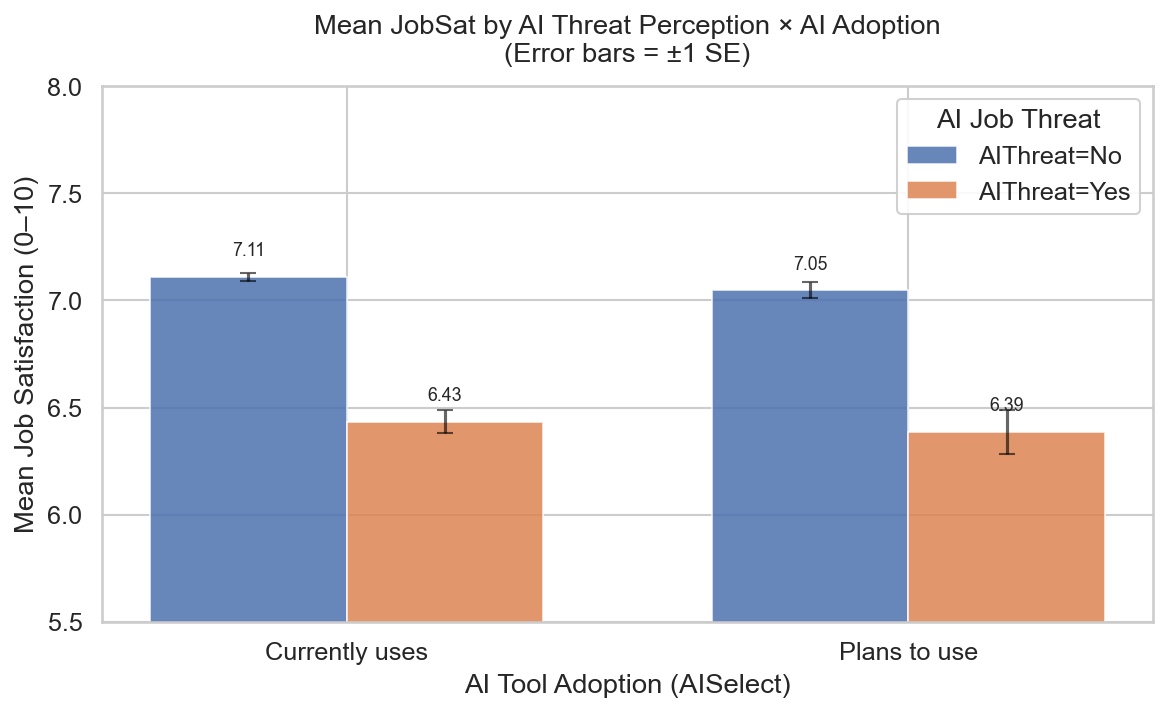
\includegraphics[width=0.68\textwidth]{fig2_grouped_bar_threat_select.png}
  \caption{Mean \textsc{JobSat} ($\pm$1~SE) by AIThreat~$\times$~AISelect.
           The AIThreat gap is consistent across AI adoption groups,
           confirming no meaningful interaction.}
  \label{fig:grouped}
\end{figure}

The interaction term AIThreat~$\times$~AISelect was non-significant
($f^2 = 0.0008$), indicating that the AIThreat effect does not depend
on whether respondents use AI tools.
As Figure~\ref{fig:grouped} shows, the gap between AIThreat=No and
AIThreat=Yes is similarly sized among current AI tool users (7.11 vs.\
6.43) and among those planning to adopt (7.02 vs.\ 6.34).

A robustness check restricted to current AI tool users ($n = 14{,}538$)
yielded $d = 0.325$ ($t = 11.89$, $p < 1.1 \times 10^{-31}$), virtually
identical to the full-sample estimate ($d = 0.327$).

% -----------------------------------------------------------------------
\section{Discussion and Conclusion}

\subsection{Interpretation}

The central finding is that perceiving AI as a job threat is associated with
lower job satisfaction among software developers (Cohen's $d = 0.33$), while
currently using AI tools is not ($d = 0.03$). This pattern is
counter-intuitive in the context of the dominant discourse, which frames
AI adoption as a driver of productivity gains and professional fulfilment.
The data suggest, instead, that the \emph{psychological stance} towards AI
matters far more than its \emph{behavioural adoption}.

This result is broadly consistent with \citet{sadeghi2024employee}, who argues
that AI's impact on employee well-being is mediated by subjective perceptions
of fairness and job security rather than by the efficiency gains the technology
delivers. It also aligns with \citet{feng2025ai}, who found that AI-related
workplace anxiety reduces life satisfaction through negative emotional states
in a cross-sectional sample of service workers.
Our study extends this evidence to the domain of software development using a
considerably larger sample.

The null effect of AISelect echoes the observation by \citet{giuntella2025ai}
that objective AI exposure (operationalised at the occupational level) does
not reduce life satisfaction. Taken together, these findings suggest a
two-tier picture: at both the macro level (occupational exposure, \citealt{giuntella2025ai})
and the individual behavioural level (tool adoption, this study), AI's
relationship with well-being is near-zero. Subjective threat perception
constitutes the critical pathway.

That the threat effect persists fully among current AI users (d = 0.33 vs.\
0.33 overall) is notable: using AI tools does not protect developers from the
negative effects of perceiving those same tools as a job threat. This points
to a form of \emph{cognitive dissonance}—continued tool adoption alongside
genuine fear of displacement—that warrants attention in both research and
organisational practice. The systematic review by \citet{soulami2024exploring}
identifies workplace autonomy and psychological health as the key mechanisms
through which AI affects employees; our findings suggest that for software
developers, perceived job insecurity is the dominant active mechanism.

\subsection{Practical Significance}

The effect is statistically robust but modest in magnitude: Cohen's $d = 0.33$
corresponds to a mean difference of 0.67 points on a 0--10 scale, and the
full model explains only 3.3\,\% of variance in job satisfaction.
This is consistent with the cross-sectional, self-report nature of the data
and the fact that job satisfaction is determined by many factors beyond
AI perceptions. The small $f^2$ value (0.011) should be clearly
communicated: AIThreat is a statistically detectable but not dominant
predictor of job satisfaction.

\subsection{Limitations}

First, the data are cross-sectional; no causal inference is possible.
Reverse causation (already dissatisfied developers may be more likely to
perceive AI as threatening) cannot be ruled out.
Second, \textsc{JobSat} was missing for 55.5\,\% of the full sample,
restricting the analytic sample to respondents with an employment context.
If dissatisfied developers systematically avoided the JobSat question,
results may underestimate the threat effect.
Third, \textsc{AIThreat} is a single binary item, providing a coarse
operationalisation of what is likely a multi-dimensional attitude.
Fourth, the survey captures perceived threat at one point in time during a
period of rapid AI adoption; results may not generalise across survey years.

\subsection{Conclusion}

Against the backdrop of widespread claims that AI tool adoption drives
developer satisfaction, this study finds that adoption behaviour is effectively
unrelated to job satisfaction ($d = 0.03$).
Perceived AI job threat, by contrast, is a consistent negative predictor
($d = 0.33$, $\beta = -0.65$, $p < 10^{-44}$) that persists across AI
adoption groups and after covariate adjustment.
Organisations seeking to improve developer well-being in the age of AI may
gain more from addressing threat perceptions—through transparent communication,
upskilling programmes, and involvement in AI rollout decisions—than from
accelerating adoption rates alone.

% -----------------------------------------------------------------------
\bibliographystyle{plainnat}
\begin{thebibliography}{9}

\bibitem[Feng et al.(2025)]{feng2025ai}
Feng, Z., Hu, C., Chen, S., Xu, J., Zhang, Y., \& Hao, M. (2025).
Impact of AI workplace anxiety on life satisfaction among service industry
employees: exploring mediating and moderating factors.
\textit{Frontiers in Psychology}, 16.
\url{https://doi.org/10.3389/fpsyg.2025.1603393}

\bibitem[Giuntella et al.(2025)]{giuntella2025ai}
Giuntella, O., Konig, J., \& Stella, L. (2025).
Artificial intelligence and the wellbeing of workers.
\textit{Scientific Reports}, 15.
\url{https://doi.org/10.1038/s41598-025-98241-3}

\bibitem[Sadeghi(2024)]{sadeghi2024employee}
Sadeghi, S. (2024).
Employee well-being in the age of AI: perceptions, concerns, behaviors,
and outcomes.
\textit{arXiv preprint} arXiv:2412.04796.
\url{https://doi.org/10.48550/arXiv.2412.04796}

\bibitem[Soulami et al.(2024)]{soulami2024exploring}
Soulami, M., Benchekroun, S., \& Galiulina, A. (2024).
Exploring how AI adoption in the workplace affects employees:
a bibliometric and systematic review.
\textit{Frontiers in Artificial Intelligence}, 7.
\url{https://doi.org/10.3389/frai.2024.1473872}

\bibitem[Vaillant et al.(2024)]{vaillant2024developers}
Vaillant, T.~S., Deveza de Almeida, F., Neto, P.~A.~M.~S., Gao, C.,
Bosch, J., \& Santana de Almeida, E. (2024).
Developers' perceptions on the impact of ChatGPT in software development:
a survey.
\textit{arXiv preprint} arXiv:2405.12195.
\url{https://doi.org/10.48550/arXiv.2405.12195}

\end{thebibliography}

\end{document}
